% Ensure that you compile using XeLaTeX !!! PDFTex has problems with some of the packages used
\documentclass[12pt]{article}
\setlength\parindent{0pt}

\usepackage{parskip}
\usepackage[margin=0.5in]{geometry}
\usepackage{fullpage}
\usepackage{moresize}
\usepackage{graphicx}
\usepackage{caption}
\usepackage{subcaption}
\usepackage{float}
\usepackage{xcolor}
\usepackage{soul}
\usepackage{fontspec}
\setmainfont{Doulos SIL}

\begin{document}

\begin{center}
\textbf{{\color{violet}{\HUGE Thursday, 4 June 2020\\}}}

\textbf{{\color{violet}{\HUGE ALL EXAMS\\}}}

\end{center}
\newpage

\begin{center}
\textbf{{\color{blue}{\HUGE START OF EXAM\\}}}

\textbf{{\color{blue}{\HUGE Student ID: 4220\\}}}

\textbf{{\color{blue}{\HUGE 11:45 AM - 12:00 noon\\}}}

\end{center}
\newpage

{\large Question 1}\\

Source: Day 5 Handout, Question 5\\

How would you look for co-occurrence restrictions between [s] and the vowels that come after it in this dataset?\\

\begin{figure}[H]
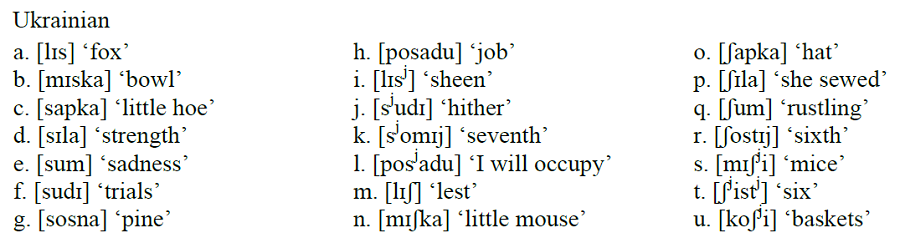
\includegraphics{../images/ukrainian.png}
\end{figure}

\newpage

{\large Question 2}\\

Source: Day 2 Discussion\\

Assuming a Standard North American English inventory, does this vowel need to have tenseness specified if you're giving a prose description? Why or why not?\\

{[u]}


\newpage

{\large Question 3}\\

Source: Day 2 Handout, Part I, Question 11\\

How would this word be transcribed?\\ Follow-up question: Why did you use symbol [X] instead of symbol [Y]?\\

<square>


\newpage

{\large Question 4}\\

Source: Day 6 Handout, Question 11\\

What do the two signs below tell you about the phonological status of \underline{handshape} in ASL, and why?\\

\begin{figure}[H]
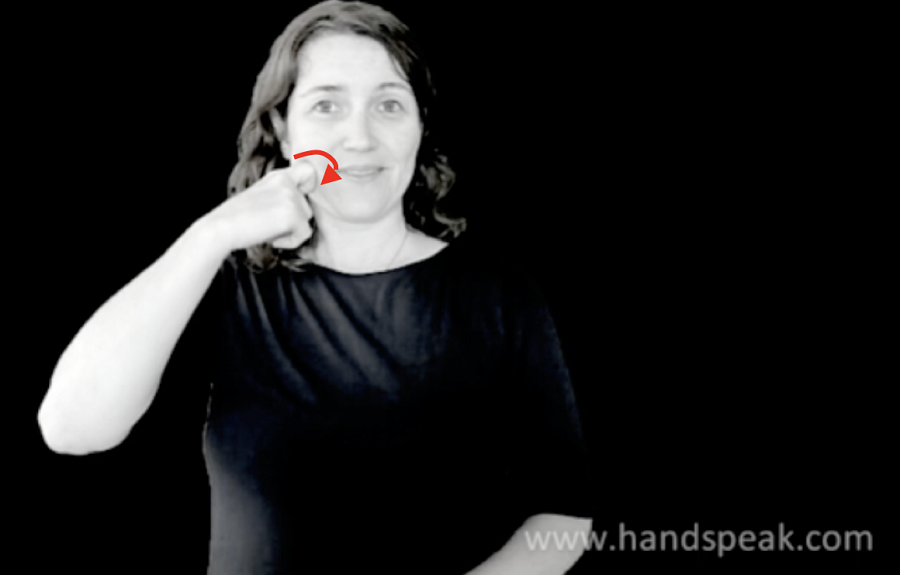
\includegraphics{../images/asl_apple.png}
\caption{APPLE}
\end{figure}
\begin{figure}[H]
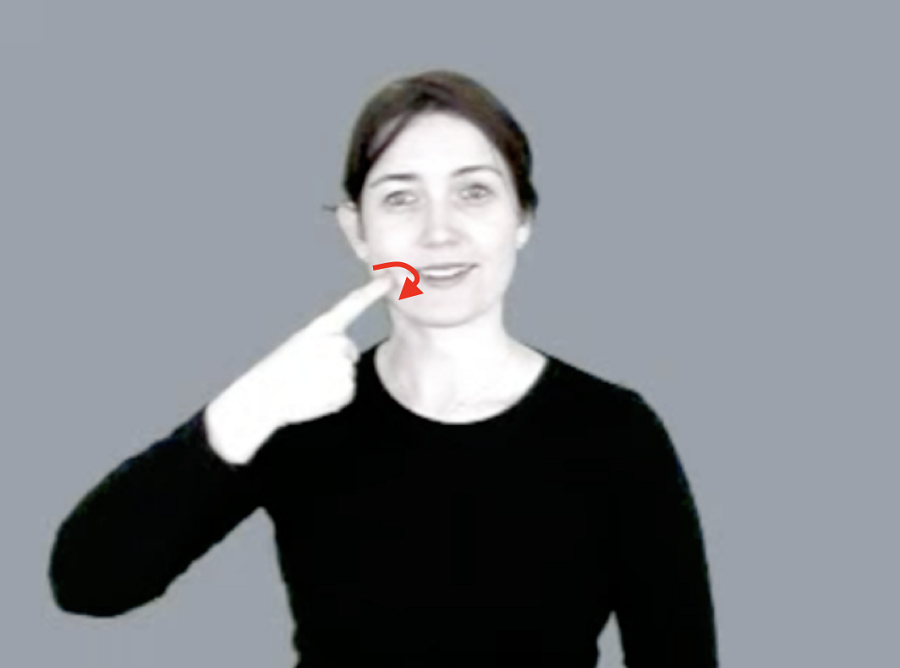
\includegraphics{../images/asl_candy.png}
\caption{CANDY}
\end{figure}

\newpage

{\large Question 5}\\

Source: Day 7 Handout, Question 2\\

Explain whether the rule below would apply to the form shown, and if so, what the effect of the rule would be. Assume the vowel inventory [i], [ɪ], [e], [ɛ], [ɑ], [u], [ʊ], [o], [ɔ].\\

/emos/

{[non-low vowel]} →  {[lax]} / \_\_ C$_0$ {[lax vowel]}


\newpage

\begin{center}
\textbf{{\color{red}{\HUGE END OF EXAM}}}\\

\end{center}
\newpage

\begin{center}
\textbf{{\color{blue}{\HUGE START OF EXAM\\}}}

\textbf{{\color{blue}{\HUGE Student ID: 3129\\}}}

\textbf{{\color{blue}{\HUGE 12:00 noon - 12:15 PM\\}}}

\end{center}
\newpage

{\large Question 1}\\

Source: Quiz 3, Question 1\\

L$_X$ (Language X) has three vowels, [i], [a], and [u]. It has bi-syllabic roots like Kikuyu. It does not allow non-identical high vowels to co-occur. Of the following nine logically possible vocalic sequences, which ones should be unattested in L$_X$? Explain why.\\

\begin{itemize} \item {[i...i]} \item {[i...a]} \item {[i...u]} \item {[a...i]} \item {[a...a]} \item {[a...u]} \item {[u...i]} \item {[u...a]} \item {[u...u]} \end{itemize}


\newpage

{\large Question 2}\\

Source: Homework 1, Question 3(b)\\

Explain why this is or is not a complete natural class in standard North American English.\\

{[ɔ]}, {[ʊ]}, {[u]}, {[oʊ]}


\newpage

{\large Question 3}\\

Source: Day 7 Handout, Question 11\\

What is the basic analysis of voiceless stops in this dataset, and what are the key pieces of evidence?\\

\begin{figure}[H]
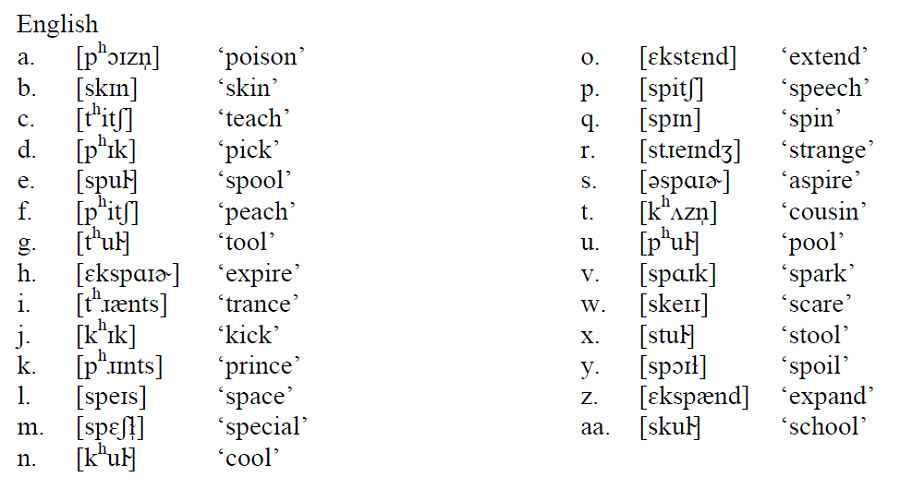
\includegraphics{../images/english11.png}
\end{figure}

\newpage

{\large Question 4}\\

Source: Day 2 Handout, Part I, Question 11\\

How would this word be transcribed?\\ Follow-up question: Why did you use symbol [X] instead of symbol [Y]?\\

<juice>


\newpage

{\large Question 5}\\

Source: Day 2 Discussion\\

Assuming a Standard North American English inventory, does this vowel need to have tenseness specified if you're giving a prose description? Why or why not?\\

{[u]}


\newpage

\begin{center}
\textbf{{\color{red}{\HUGE END OF EXAM}}}\\

\end{center}
\newpage

\begin{center}
\textbf{{\color{blue}{\HUGE START OF EXAM\\}}}

\textbf{{\color{blue}{\HUGE Student ID: 7661\\}}}

\textbf{{\color{blue}{\HUGE 12:15 PM - 12:30 PM\\}}}

\end{center}
\newpage

{\large Question 1}\\

Source: Quiz 3, Question 1\\

L$_X$ (Language X) has three vowels, [i], [a], and [u]. It has bi-syllabic roots like Kikuyu. It does not allow non-identical high vowels to co-occur. Of the following nine logically possible vocalic sequences, which ones should be unattested in L$_X$? Explain why.\\

\begin{itemize} \item {[i...i]} \item {[i...a]} \item {[i...u]} \item {[a...i]} \item {[a...a]} \item {[a...u]} \item {[u...i]} \item {[u...a]} \item {[u...u]} \end{itemize}


\newpage

{\large Question 2}\\

Source: Day 7 Handout, Question 9\\

What is the basic analysis of vowel length in this dataset, and what are the key pieces of evidence?\\

\begin{figure}[H]
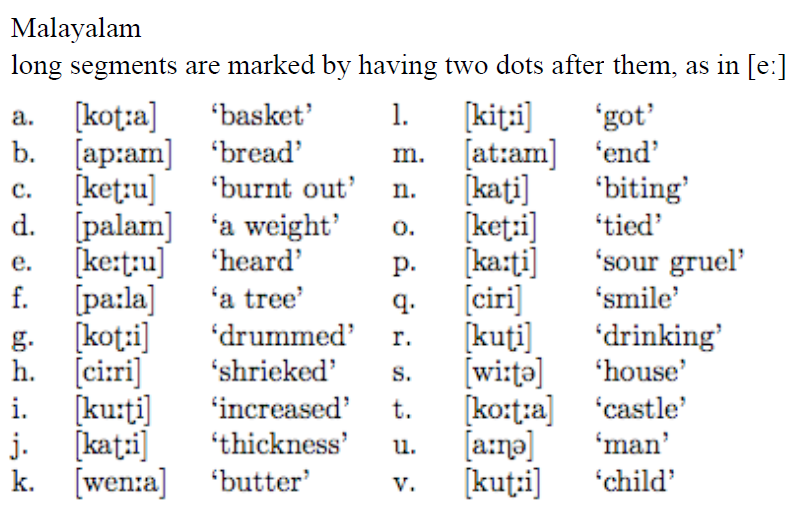
\includegraphics{../images/malayalam.png}
\end{figure}

\newpage

{\large Question 3}\\

Source: Day 6 Handout, Question 7\\

Explain how you would determine the phonological relationship between these two sounds (given below) in this dataset.\\

{[s]} and {[z]}

\begin{figure}[H]
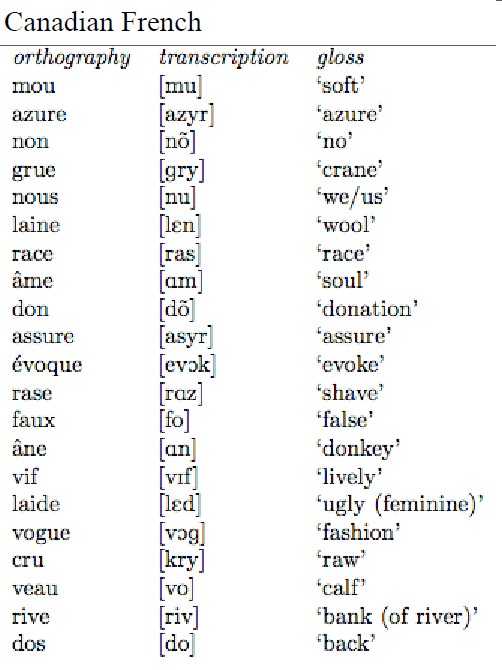
\includegraphics{../images/canadianfrench.png}
\end{figure}

\newpage

{\large Question 4}\\

Source: Day 2 Discussion\\

Assuming a Standard North American English inventory, does this vowel need to have tenseness specified if you're giving a prose description? Why or why not?\\

{[ɑ]}


\newpage

{\large Question 5}\\

Source: Day 2 Handout, Part I, Question 11\\

How would this word be transcribed?\\ Follow-up question: Why did you use symbol [X] instead of symbol [Y]?\\

<toy>


\newpage

\begin{center}
\textbf{{\color{red}{\HUGE END OF EXAM}}}\\

\end{center}
\newpage

\begin{center}
\textbf{{\color{blue}{\HUGE START OF EXAM\\}}}

\textbf{{\color{blue}{\HUGE Student ID: 3684\\}}}

\textbf{{\color{blue}{\HUGE 12:30 - 12:45 PM\\}}}

\end{center}
\newpage

{\large Question 1}\\

Source: Quiz 3, Question 2\\

L$_X$ has tri-syllabic roots. If L$_X$ does not allow non-identical high vowels to co-occur, which one of the following tri-syllabic vocalic sequences do you predict to be unattested in L$_X$? Explain why.\\

\begin{itemize} \item {[u...i...a]} \item {[a...i...a]} \item {[u...u...a]} \item {[a...i...i]} \end{itemize}


\newpage

{\large Question 2}\\

Source: Day 7 Handout, Question 11\\

What is the basic analysis of voiceless stops in this dataset, and what are the key pieces of evidence?\\

\begin{figure}[H]
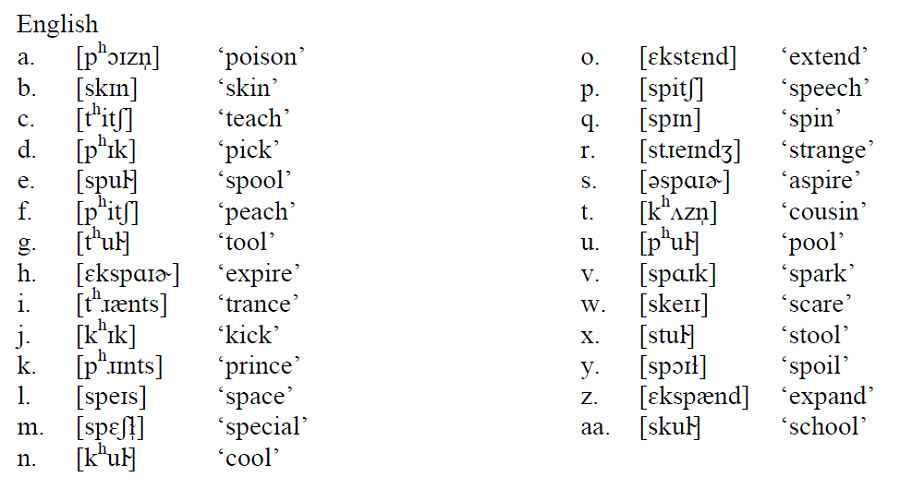
\includegraphics{../images/english11.png}
\end{figure}

\newpage

{\large Question 3}\\

Source: Homework 1, Question 3(b)\\

Explain why this is or is not a complete natural class in standard North American English.\\

{[b]}, {[n]}, {[ɡ]}, {[ʒ]}, {[v]}


\newpage

{\large Question 4}\\

Source: Day 2 Handout, Part I, Question 11\\

How would this word be transcribed?\\ Follow-up question: Why did you use symbol [X] instead of symbol [Y]?\\

<bird>


\newpage

{\large Question 5}\\

Source: Day 2 Handout, Part I, Question 11\\

How would this word be transcribed?\\ Follow-up question: Why did you use symbol [X] instead of symbol [Y]?\\

<segment>


\newpage

\begin{center}
\textbf{{\color{red}{\HUGE END OF EXAM}}}\\

\end{center}
\newpage

\begin{center}
\textbf{{\color{blue}{\HUGE START OF EXAM\\}}}

\textbf{{\color{blue}{\HUGE Student ID: 3737\\}}}

\textbf{{\color{blue}{\HUGE 12:45 - 1:00 PM\\}}}

\end{center}
\newpage

{\large Question 1}\\

Source: Day 5 Handout, Question 5\\

How would you look for co-occurrence restrictions between [s] and the vowels that come after it in this dataset?\\

\begin{figure}[H]
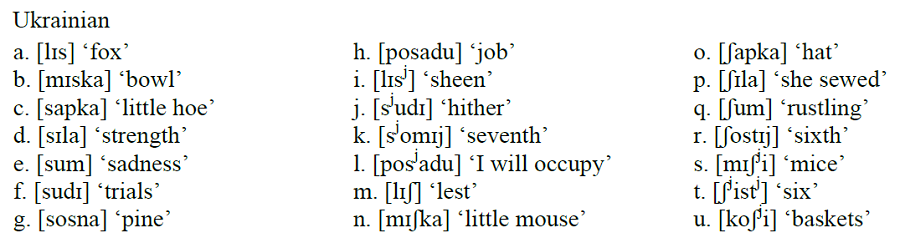
\includegraphics{../images/ukrainian.png}
\end{figure}

\newpage

{\large Question 2}\\

Source: Day 7 Handout, Question 12\\

What is the basic analysis of oral and nasal vowels in this dataset, and what are the key pieces of evidence?\\

\begin{figure}[H]
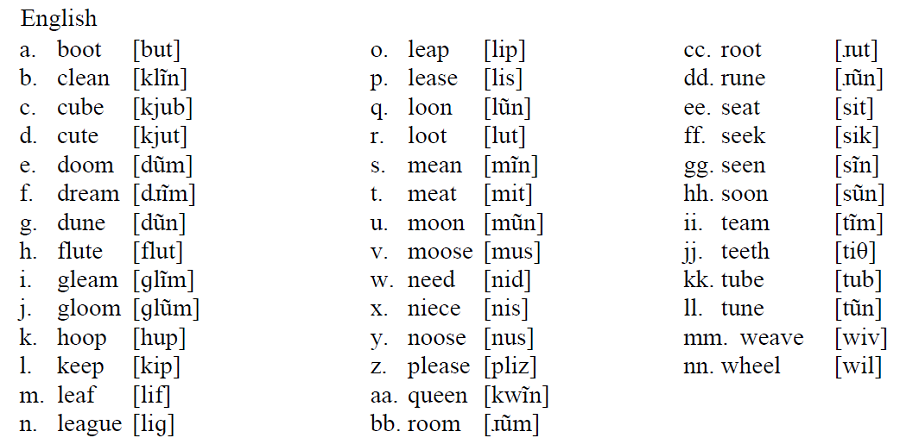
\includegraphics{../images/english12.png}
\end{figure}

\newpage

{\large Question 3}\\

Source: Day 2 Handout, Part I, Question 11\\

How would this word be transcribed?\\ Follow-up question: Why did you use symbol [X] instead of symbol [Y]?\\

<bird>


\newpage

{\large Question 4}\\

Source: Day 4 Handout, Question 2(iv)\\

Explain how you would figure out the Swahili word for this English gloss.\\

‘I wanted them.’

\begin{figure}[H]
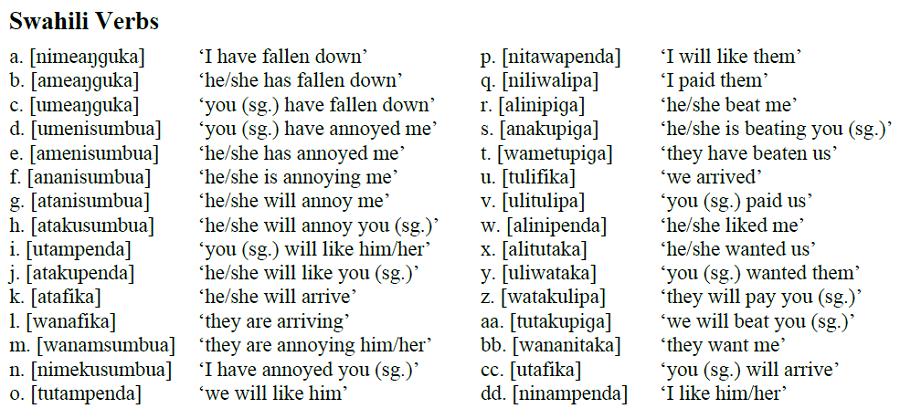
\includegraphics{../images/swahiliverbs.png}
\end{figure}

\newpage

{\large Question 5}\\

Source: Day 2 Handout, Part II, Question 13\\

Explain why this image does or does not match the description.\\

\begin{itemize} \item A one-handed sign. \item Location: In front of signer’s chin. \item Handshape: Starts with an “L” shape; proximal joint of index finger folds down during the sign. \item Movement: Hand starts on far side of signer’s body and moves horizontally straight across. \end{itemize}

\begin{figure}[H]
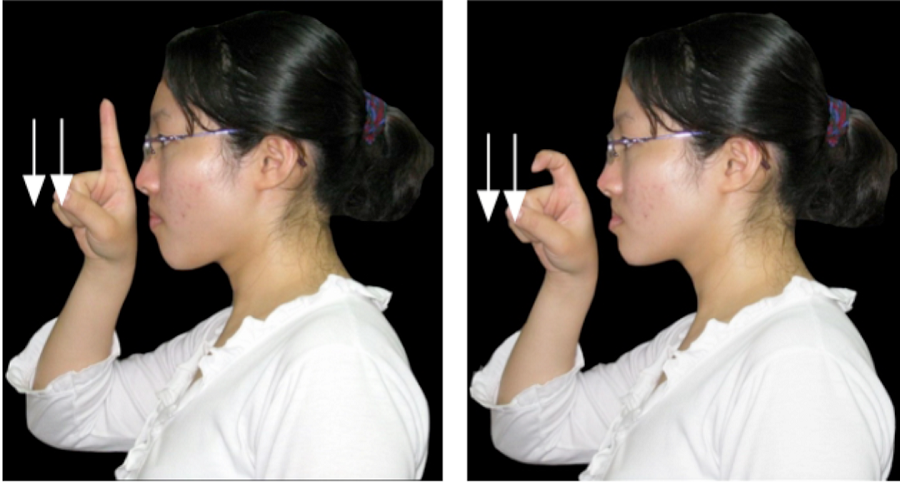
\includegraphics{../images/taiwansign_jealous.png}
\caption{JEALOUS}
\end{figure}

\newpage

\begin{center}
\textbf{{\color{red}{\HUGE END OF EXAM}}}\\

\end{center}
\newpage

\begin{center}
\textbf{{\color{blue}{\HUGE START OF EXAM\\}}}

\textbf{{\color{blue}{\HUGE Student ID: 5824\\}}}

\textbf{{\color{blue}{\HUGE 1:00 - 1:15 PM\\}}}

\end{center}
\newpage

{\large Question 1}\\

Source: Day 5 Handout, Question 3\\

What evidence is there that there is a pattern in these data, assuming that these are the only CV and VC sequences that occur in some language?\\

{[sa]}, {[ʃi]}, {[za]}, {[ʒi]}, {[as]}, {[iʃ]}, {[az]}, {[iʒ]}


\newpage

{\large Question 2}\\

Source: Day 2 Handout, Part I, Question 11\\

How would this word be transcribed?\\ Follow-up question: Why did you use symbol [X] instead of symbol [Y]?\\

<finger>


\newpage

{\large Question 3}\\

Source: Quiz 2, Question 6\\

In the pronunciation of this word, which sounds are obstruents and which are sonorants?\\

<sonorant>


\newpage

{\large Question 4}\\

Source: Day 2 Handout, Part I, Question 11\\

How would this word be transcribed?\\ Follow-up question: Why did you use symbol [X] instead of symbol [Y]?\\

<toy>


\newpage

{\large Question 5}\\

Source: Day 6 Handout, Question 11\\

What do the two signs below tell you about the phonological status of \underline{handshape} in ASL, and why?\\

\begin{figure}[H]
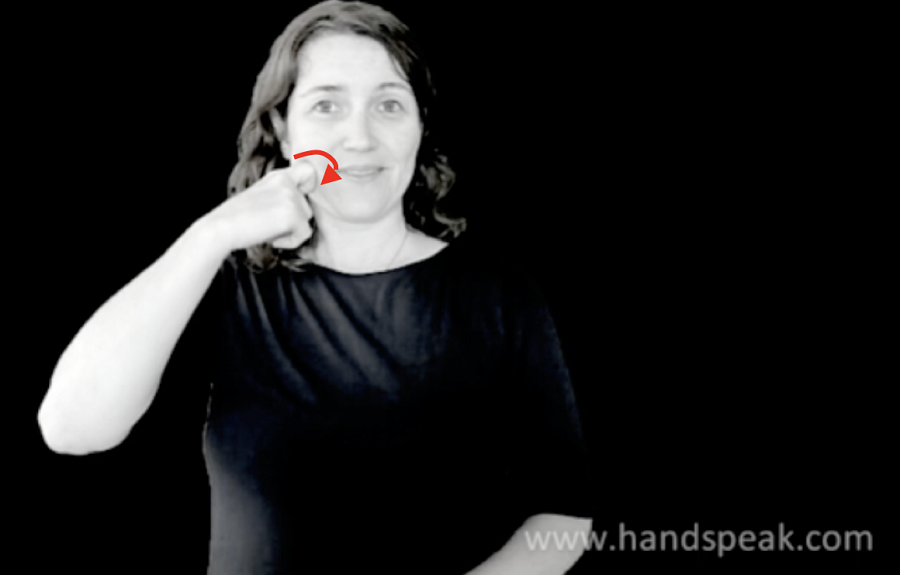
\includegraphics{../images/asl_apple.png}
\caption{APPLE}
\end{figure}
\begin{figure}[H]
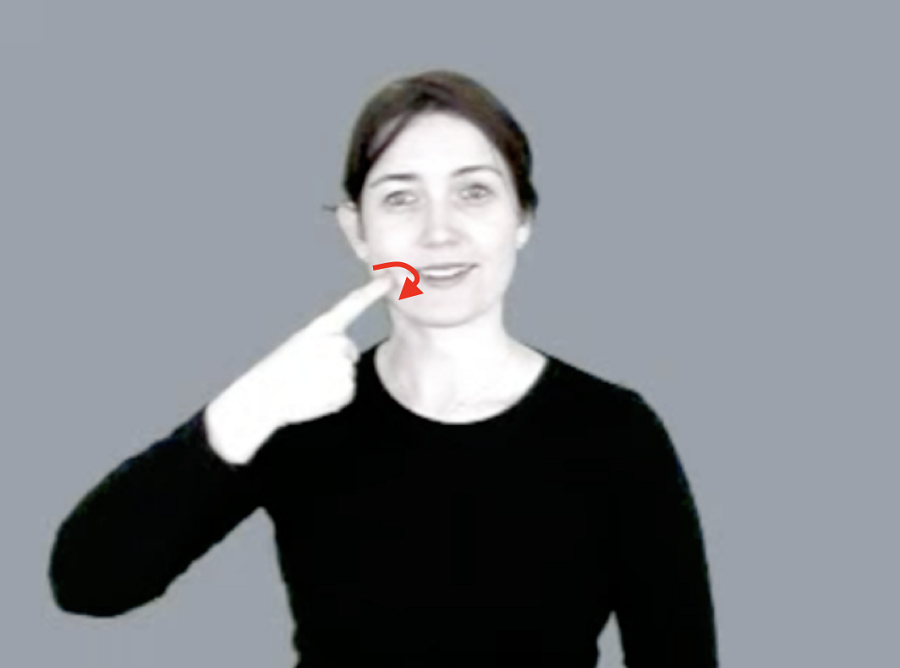
\includegraphics{../images/asl_candy.png}
\caption{CANDY}
\end{figure}

\newpage

\begin{center}
\textbf{{\color{red}{\HUGE END OF EXAM}}}\\

\end{center}
\newpage

\begin{center}
\textbf{{\color{blue}{\HUGE START OF EXAM\\}}}

\textbf{{\color{blue}{\HUGE Student ID: 1743\\}}}

\textbf{{\color{blue}{\HUGE 1:15 - 1:30 PM\\}}}

\end{center}
\newpage

{\large Question 1}\\

Source: Day 5 Handout, Question 3\\

What evidence is there that there is a pattern in these data, assuming that these are the only CV and VC sequences that occur in some language?\\

{[sa]}, {[ʃi]}, {[za]}, {[ʒi]}, {[as]}, {[iʃ]}, {[az]}, {[iʒ]}


\newpage

{\large Question 2}\\

Source: Day 2 Handout, Part I, Question 11\\

How would this word be transcribed?\\ Follow-up question: Why did you use symbol [X] instead of symbol [Y]?\\

<toy>


\newpage

{\large Question 3}\\

Source: Day 2 Discussion\\

Assuming a Standard North American English inventory, does this vowel need to have tenseness specified if you're giving a prose description? Why or why not?\\

{[æ]}


\newpage

{\large Question 4}\\

Source: Day 6 Handout, Question 11\\

What do the two signs below tell you about the phonological status of \underline{handshape} in ASL, and why?\\

\begin{figure}[H]
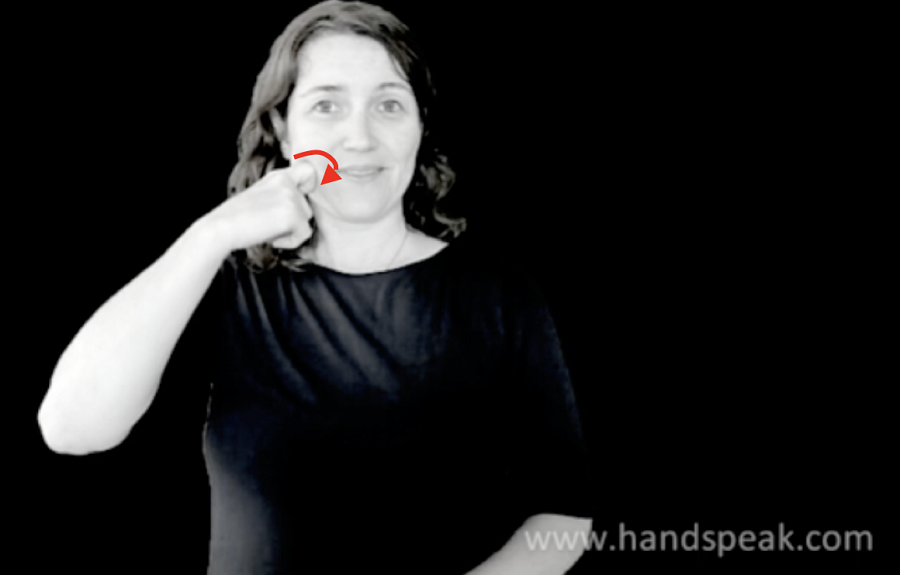
\includegraphics{../images/asl_apple.png}
\caption{APPLE}
\end{figure}
\begin{figure}[H]
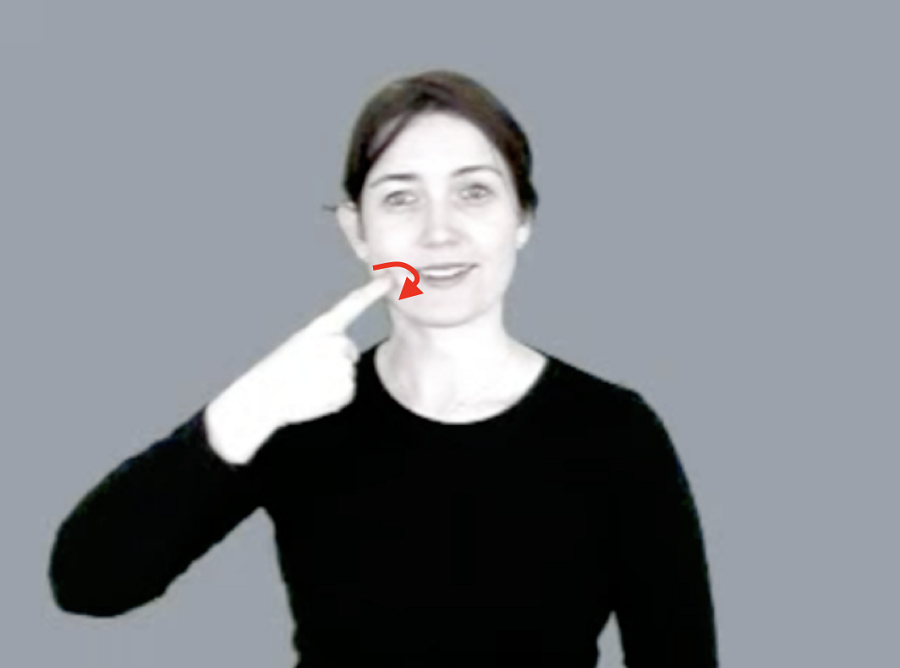
\includegraphics{../images/asl_candy.png}
\caption{CANDY}
\end{figure}

\newpage

{\large Question 5}\\

Source: Day 2 Discussion\\

Assuming a Standard North American English inventory, does this vowel need to have tenseness specified if you're giving a prose description? Why or why not?\\

{[u]}


\newpage

\begin{center}
\textbf{{\color{red}{\HUGE END OF EXAM}}}\\

\end{center}
\newpage

\begin{center}
\textbf{{\color{blue}{\HUGE START OF EXAM\\}}}

\textbf{{\color{blue}{\HUGE Student ID: 2014\\}}}

\textbf{{\color{blue}{\HUGE 1:30 - 1:45 PM\\}}}

\end{center}
\newpage

{\large Question 1}\\

Source: Day 5 Handout, Question 3\\

What evidence is there that there is a pattern in these data, assuming that these are the only CV and VC sequences that occur in some language?\\

{[sa]}, {[ʃi]}, {[za]}, {[ʒi]}, {[as]}, {[iʃ]}, {[az]}, {[iʒ]}


\newpage

{\large Question 2}\\

Source: Homework 2, Question 2\\

Why should the following two questions have the same answer?\\

\begin{itemize} \item Given the vowel system of Jita, how many bi-syllabic root types would you expect to find for nouns in the language? \item Assuming that the vowel inventory is the same in verbs as it is in nouns, how many bisyllabic root types would you expect to find for verbs in the language? \end{itemize}


\newpage

{\large Question 3}\\

Source: Day 2 Handout, Part I, Question 11\\

How would this word be transcribed?\\ Follow-up question: Why did you use symbol [X] instead of symbol [Y]?\\

<nice>


\newpage

{\large Question 4}\\

Source: Quiz 2, Question 6\\

In the pronunciation of this word, which sounds are obstruents and which are sonorants?\\

<minimal>


\newpage

{\large Question 5}\\

Source: Day 7 Handout, Question 9\\

What is the basic analysis of vowel length in this dataset, and what are the key pieces of evidence?\\

\begin{figure}[H]
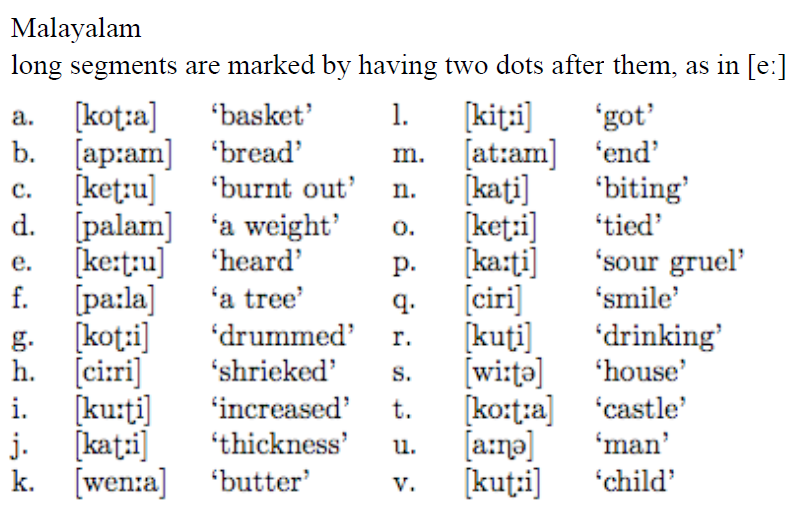
\includegraphics{../images/malayalam.png}
\end{figure}

\newpage

\begin{center}
\textbf{{\color{red}{\HUGE END OF EXAM}}}\\

\end{center}
\newpage

\begin{center}
\textbf{{\color{blue}{\HUGE START OF EXAM\\}}}

\textbf{{\color{blue}{\HUGE Student ID: 9657\\}}}

\textbf{{\color{blue}{\HUGE 1:45 - 2:00 PM\\}}}

\end{center}
\newpage

{\large Question 1}\\

Source: Quiz 3, Question 1\\

L$_X$ (Language X) has three vowels, [i], [a], and [u]. It has bi-syllabic roots like Kikuyu. It does not allow non-identical high vowels to co-occur. Of the following nine logically possible vocalic sequences, which ones should be unattested in L$_X$? Explain why.\\

\begin{itemize} \item {[i...i]} \item {[i...a]} \item {[i...u]} \item {[a...i]} \item {[a...a]} \item {[a...u]} \item {[u...i]} \item {[u...a]} \item {[u...u]} \end{itemize}


\newpage

{\large Question 2}\\

Source: Day 2 Handout, Part I, Question 11\\

How would this word be transcribed?\\ Follow-up question: Why did you use symbol [X] instead of symbol [Y]?\\

<goat>


\newpage

{\large Question 3}\\

Source: Day 4 Handout, Question 2(iv)\\

Explain how you would figure out the Swahili word for this English gloss.\\

‘I like you (sg.).’

\begin{figure}[H]
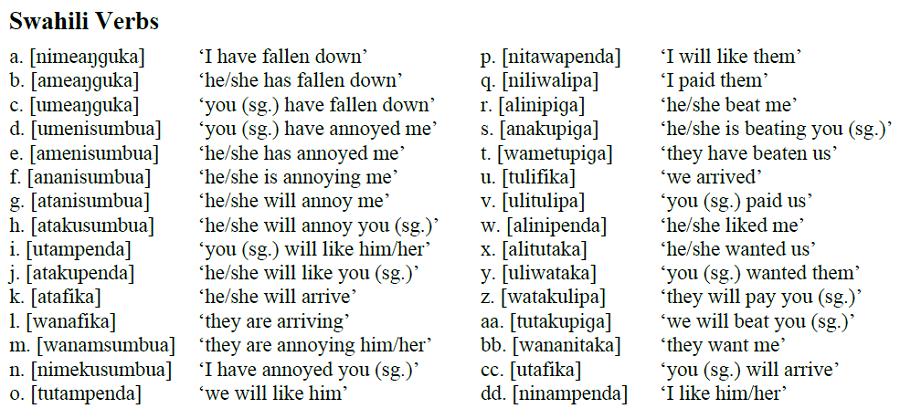
\includegraphics{../images/swahiliverbs.png}
\end{figure}

\newpage

{\large Question 4}\\

Source: Day 7 Handout, Question 9\\

What is the basic analysis of vowel length in this dataset, and what are the key pieces of evidence?\\

\begin{figure}[H]
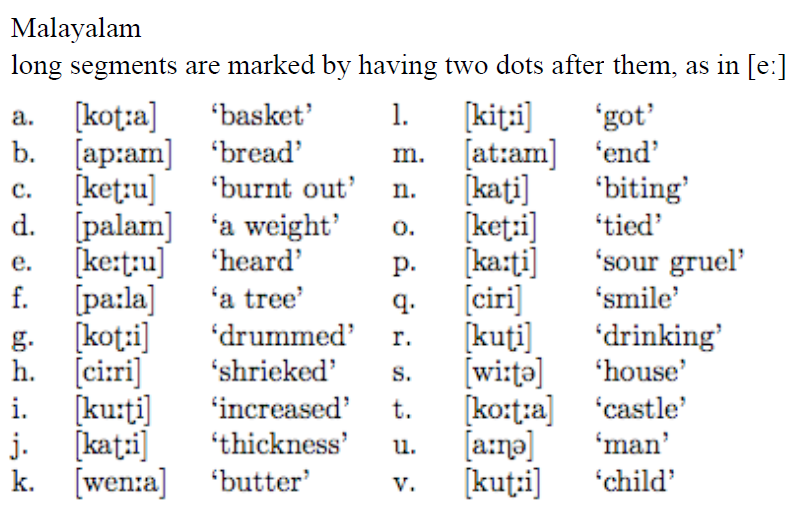
\includegraphics{../images/malayalam.png}
\end{figure}

\newpage

{\large Question 5}\\

Source: Quiz 2, Question 6\\

In the pronunciation of this word, which sounds are obstruents and which are sonorants?\\

<obstruent>


\newpage

\begin{center}
\textbf{{\color{red}{\HUGE END OF EXAM}}}\\

\end{center}
\newpage

\begin{center}
\textbf{{\color{blue}{\HUGE START OF EXAM\\}}}

\textbf{{\color{blue}{\HUGE Student ID: 9246\\}}}

\textbf{{\color{blue}{\HUGE 2:00 - 2:15 PM\\}}}

\end{center}
\newpage

{\large Question 1}\\

Source: Quiz 3, Question 1\\

L$_X$ (Language X) has three vowels, [i], [a], and [u]. It has bi-syllabic roots like Kikuyu. It does not allow non-identical high vowels to co-occur. Of the following nine logically possible vocalic sequences, which ones should be unattested in L$_X$? Explain why.\\

\begin{itemize} \item {[i...i]} \item {[i...a]} \item {[i...u]} \item {[a...i]} \item {[a...a]} \item {[a...u]} \item {[u...i]} \item {[u...a]} \item {[u...u]} \end{itemize}


\newpage

{\large Question 2}\\

Source: Day 7 Handout, Question 12\\

What is the basic analysis of oral and nasal vowels in this dataset, and what are the key pieces of evidence?\\

\begin{figure}[H]
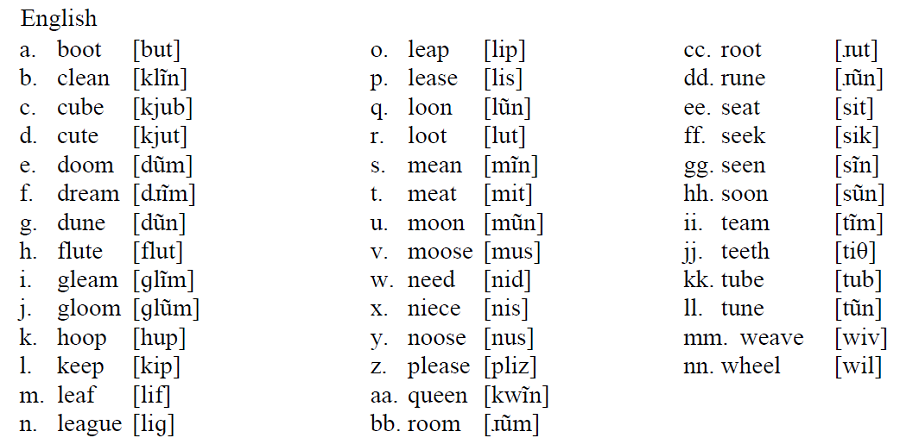
\includegraphics{../images/english12.png}
\end{figure}

\newpage

{\large Question 3}\\

Source: Day 2 Handout, Part II, Question 7\\

Is the symbol given a reasonable way to transcribe any of the sounds described below? If so, which one? If not, why not?\\

{[n]}

\begin{itemize} \item voiceless palatal affricate \item voiced velar nasal \item voiceless glottal fricative \item voiced labiodental fricative \item voiced interdental fricative \item voiced palatal fricative \end{itemize}


\newpage

{\large Question 4}\\

Source: Day 2 Handout, Part I, Question 11\\

How would this word be transcribed?\\ Follow-up question: Why did you use symbol [X] instead of symbol [Y]?\\

<goat>


\newpage

{\large Question 5}\\

Source: Day 2 Handout, Part I, Question 11\\

How would this word be transcribed?\\ Follow-up question: Why did you use symbol [X] instead of symbol [Y]?\\

<little>


\newpage

\begin{center}
\textbf{{\color{red}{\HUGE END OF EXAM}}}\\

\end{center}
\newpage

\begin{center}
\textbf{{\color{blue}{\HUGE START OF EXAM\\}}}

\textbf{{\color{blue}{\HUGE Student ID: 4465\\}}}

\textbf{{\color{blue}{\HUGE 2:30 - 2:45 PM\\}}}

\end{center}
\newpage

{\large Question 1}\\

Source: Quiz 3, Question 1\\

L$_X$ (Language X) has three vowels, [i], [a], and [u]. It has bi-syllabic roots like Kikuyu. It does not allow non-identical high vowels to co-occur. Of the following nine logically possible vocalic sequences, which ones should be unattested in L$_X$? Explain why.\\

\begin{itemize} \item {[i...i]} \item {[i...a]} \item {[i...u]} \item {[a...i]} \item {[a...a]} \item {[a...u]} \item {[u...i]} \item {[u...a]} \item {[u...u]} \end{itemize}


\newpage

{\large Question 2}\\

Source: Day 2 Handout, Part I, Question 11\\

How would this word be transcribed?\\ Follow-up question: Why did you use symbol [X] instead of symbol [Y]?\\

<vacuum>


\newpage

{\large Question 3}\\

Source: Day 6 Handout, Question 11\\

What do the two signs below tell you about the phonological status of \underline{handshape} in ASL, and why?\\

\begin{figure}[H]
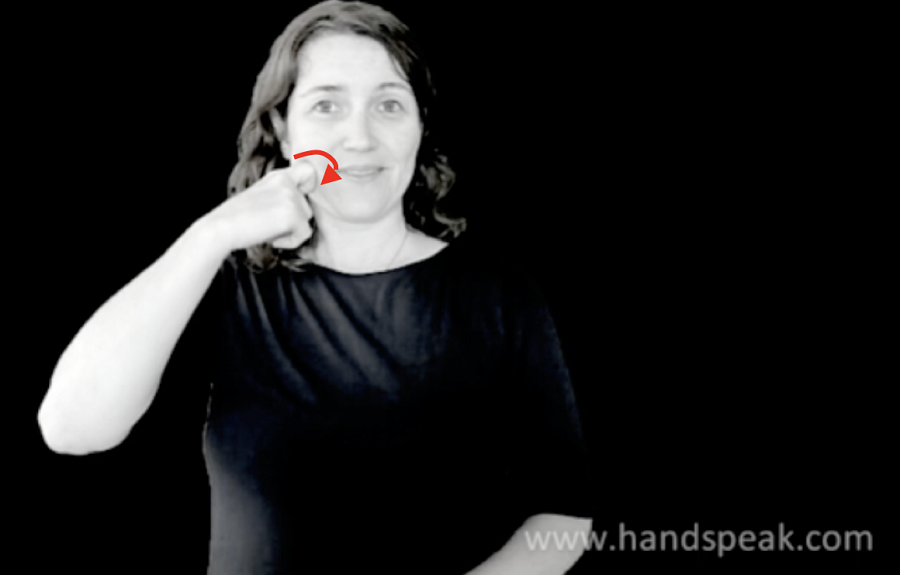
\includegraphics{../images/asl_apple.png}
\caption{APPLE}
\end{figure}
\begin{figure}[H]
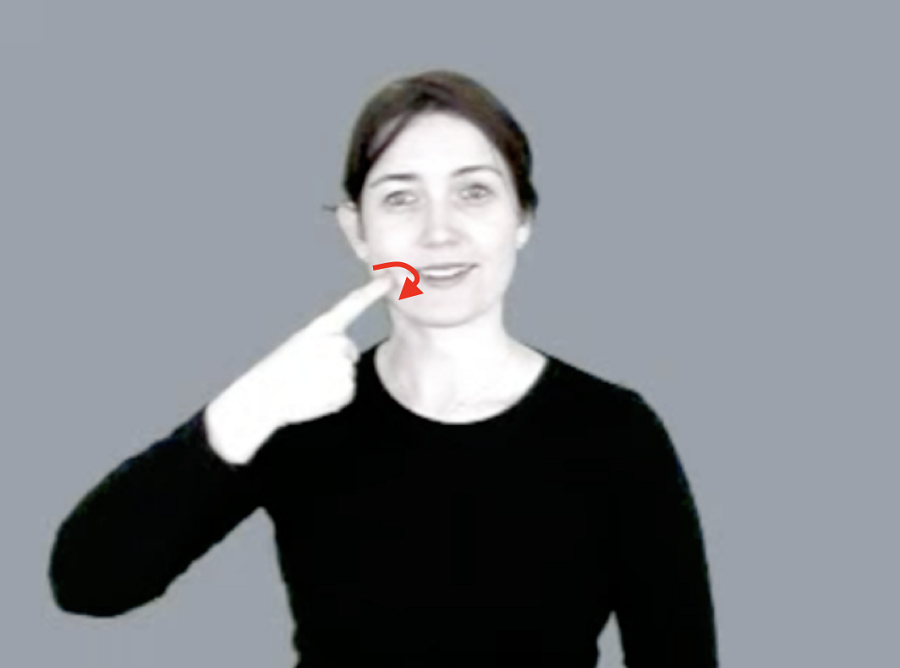
\includegraphics{../images/asl_candy.png}
\caption{CANDY}
\end{figure}

\newpage

{\large Question 4}\\

Source: Day 2 Handout, Part II, Question 7\\

Is the symbol given a reasonable way to transcribe any of the sounds described below? If so, which one? If not, why not?\\

{[ʃ]}

\begin{itemize} \item voiceless palatal affricate \item voiced velar nasal \item voiceless glottal fricative \item voiced labiodental fricative \item voiced interdental fricative \item voiced palatal fricative \end{itemize}


\newpage

{\large Question 5}\\

Source: Day 6 Handout, Question 7\\

Explain how you would determine the phonological relationship between these two sounds (given below) in this dataset.\\

{[d]} and {[n]}

\begin{figure}[H]
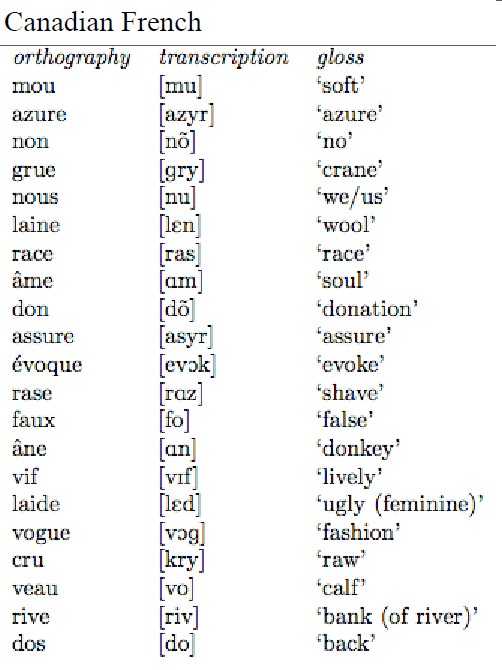
\includegraphics{../images/canadianfrench.png}
\end{figure}

\newpage

\begin{center}
\textbf{{\color{red}{\HUGE END OF EXAM}}}\\

\end{center}
\newpage

\begin{center}
\textbf{{\color{blue}{\HUGE START OF EXAM\\}}}

\textbf{{\color{blue}{\HUGE Student ID: 2931\\}}}

\textbf{{\color{blue}{\HUGE 2:45 - 3:00 PM\\}}}

\end{center}
\newpage

{\large Question 1}\\

Source: Day 5 Handout, Question 5\\

How would you look for co-occurrence restrictions between [s] and the vowels that come after it in this dataset?\\

\begin{figure}[H]
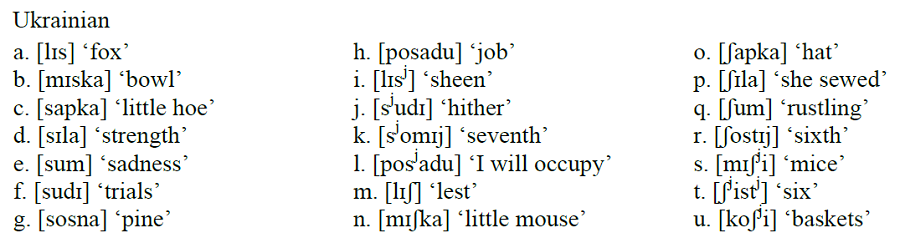
\includegraphics{../images/ukrainian.png}
\end{figure}

\newpage

{\large Question 2}\\

Source: Day 2 Handout\\

Is this a reasonable transcription of this word? Explain why.\\

<mouse>: {[mɔɪs]}


\newpage

{\large Question 3}\\

Source: Day 2 Handout, Part II, Question 9\\

Explain how to figure out what the sound being produced is in this diagram.\\

\begin{figure}[H]
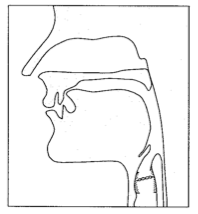
\includegraphics{../images/sagittal_z.png}
\end{figure}

\newpage

{\large Question 4}\\

Source: Day 7 Handout, Question 9\\

What is the basic analysis of vowel length in this dataset, and what are the key pieces of evidence?\\

\begin{figure}[H]
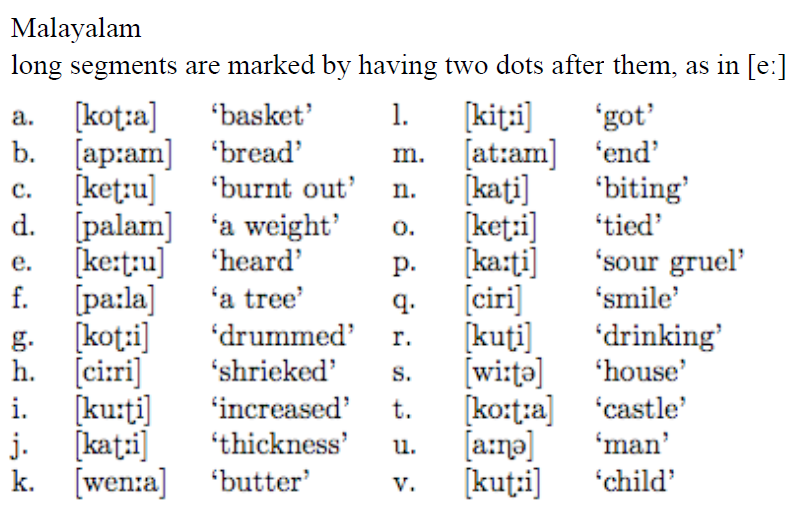
\includegraphics{../images/malayalam.png}
\end{figure}

\newpage

{\large Question 5}\\

Source: Day 2 Handout, Part I, Question 2\\

Explain why people might legitimately disagree about how many sounds this particular word contains.\\

<they>


\newpage

\begin{center}
\textbf{{\color{red}{\HUGE END OF EXAM}}}\\

\end{center}
\newpage

\begin{center}
\textbf{{\color{blue}{\HUGE START OF EXAM\\}}}

\textbf{{\color{blue}{\HUGE Student ID: 8742\\}}}

\textbf{{\color{blue}{\HUGE 3:00 - 3:15 PM\\}}}

\end{center}
\newpage

{\large Question 1}\\

Source: Quiz 3, Question 1\\

L$_X$ (Language X) has three vowels, [i], [a], and [u]. It has bi-syllabic roots like Kikuyu. It does not allow non-identical high vowels to co-occur. Of the following nine logically possible vocalic sequences, which ones should be unattested in L$_X$? Explain why.\\

\begin{itemize} \item {[i...i]} \item {[i...a]} \item {[i...u]} \item {[a...i]} \item {[a...a]} \item {[a...u]} \item {[u...i]} \item {[u...a]} \item {[u...u]} \end{itemize}


\newpage

{\large Question 2}\\

Source: Day 2 Handout, Part I, Question 11\\

How would this word be transcribed?\\ Follow-up question: Why did you use symbol [X] instead of symbol [Y]?\\

<square>


\newpage

{\large Question 3}\\

Source: Day 6 Handout, Question 11\\

What do the two signs below tell you about the phonological status of \underline{handshape} in ASL, and why?\\

\begin{figure}[H]
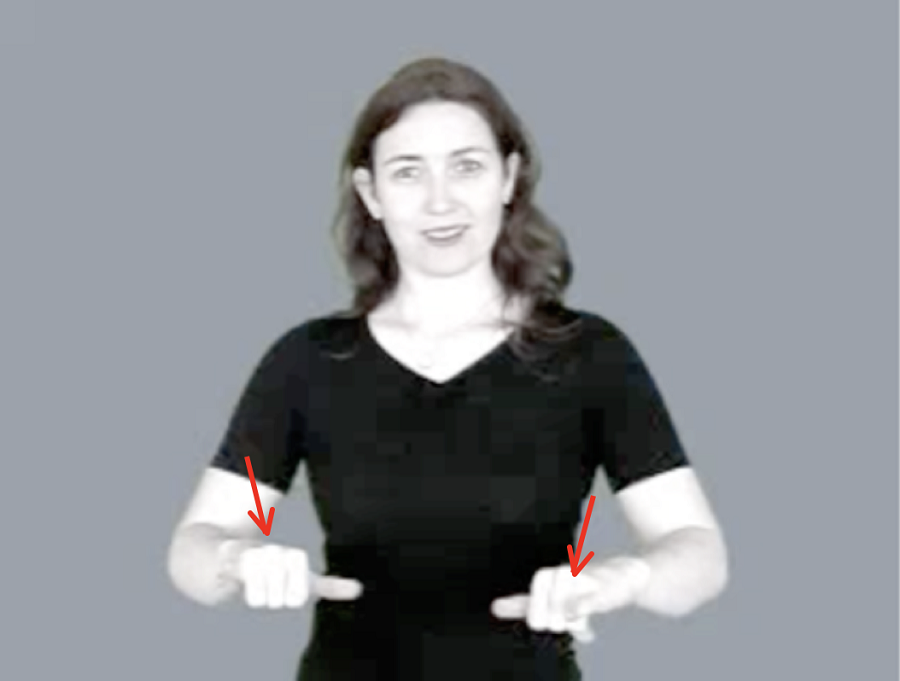
\includegraphics{../images/asl_stay.png}
\caption{STAY}
\end{figure}
\begin{figure}[H]
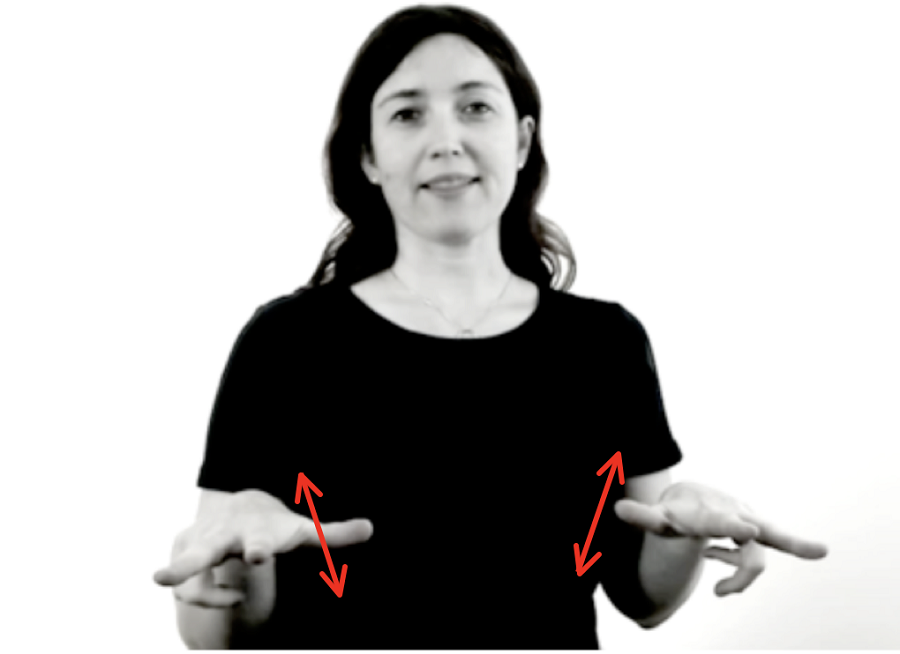
\includegraphics{../images/asl_awkward.png}
\caption{AWKWARD}
\end{figure}

\newpage

{\large Question 4}\\

Source: Homework 1, Question 3(b)\\

Explain why this is or is not a complete natural class in standard North American English.\\

{[f]}, {[s]}, {[ʃ]}


\newpage

{\large Question 5}\\

Source: Quiz 2, Question 6\\

In the pronunciation of this word, which sounds are obstruents and which are sonorants?\\

<fricative>


\newpage

\begin{center}
\textbf{{\color{red}{\HUGE END OF EXAM}}}\\

\end{center}
\newpage

\begin{center}
\textbf{{\color{blue}{\HUGE START OF EXAM\\}}}

\textbf{{\color{blue}{\HUGE Student ID: 4199\\}}}

\textbf{{\color{blue}{\HUGE 3:15 - 3:30 PM\\}}}

\end{center}
\newpage

{\large Question 1}\\

Source: Quiz 3, Question 1\\

L$_X$ (Language X) has three vowels, [i], [a], and [u]. It has bi-syllabic roots like Kikuyu. It does not allow non-identical high vowels to co-occur. Of the following nine logically possible vocalic sequences, which ones should be unattested in L$_X$? Explain why.\\

\begin{itemize} \item {[i...i]} \item {[i...a]} \item {[i...u]} \item {[a...i]} \item {[a...a]} \item {[a...u]} \item {[u...i]} \item {[u...a]} \item {[u...u]} \end{itemize}


\newpage

{\large Question 2}\\

Source: Day 2 Handout, Part I, Question 11\\

How would this word be transcribed?\\ Follow-up question: Why did you use symbol [X] instead of symbol [Y]?\\

<nice>


\newpage

{\large Question 3}\\

Source: Homework 2, Question 1\\

What would this Klingon phrase below be in English? How do you know?\\

{[pɑdɑq]}

\begin{figure}[H]
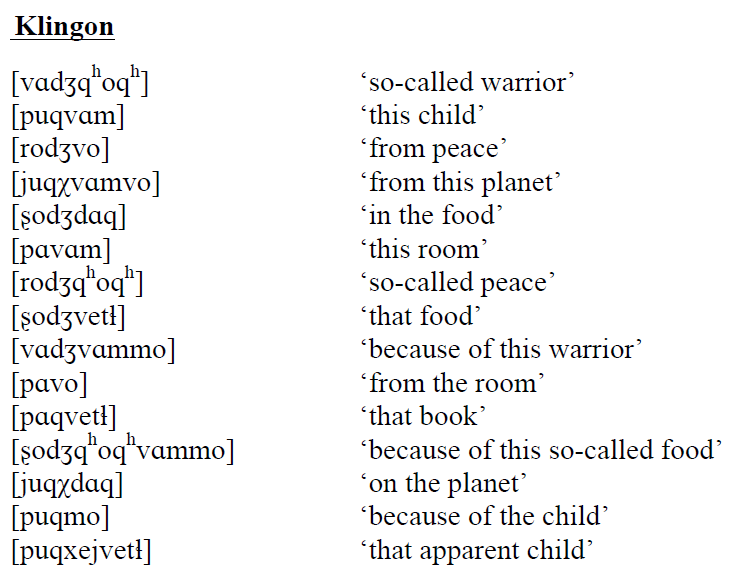
\includegraphics{../images/klingon.png}
\end{figure}

\newpage

{\large Question 4}\\

Source: Day 2 Discussion\\

Assuming a Standard North American English inventory, does this vowel need to have tenseness specified if you're giving a prose description? Why or why not?\\

{[ɛ]}


\newpage

{\large Question 5}\\

Source: Day 6 Handout, Question 11\\

What do the two signs below tell you about the phonological status of \underline{handshape} in ASL, and why?\\

\begin{figure}[H]
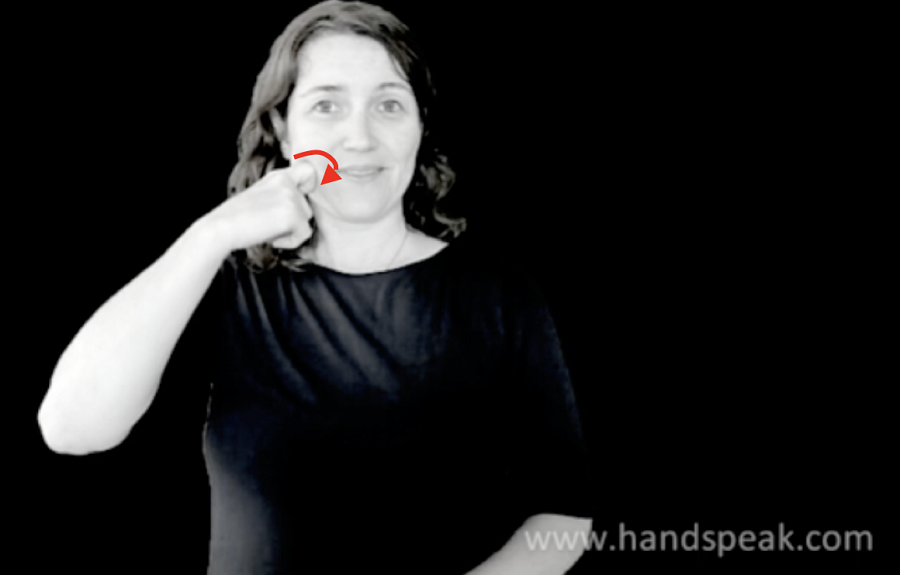
\includegraphics{../images/asl_apple.png}
\caption{APPLE}
\end{figure}
\begin{figure}[H]
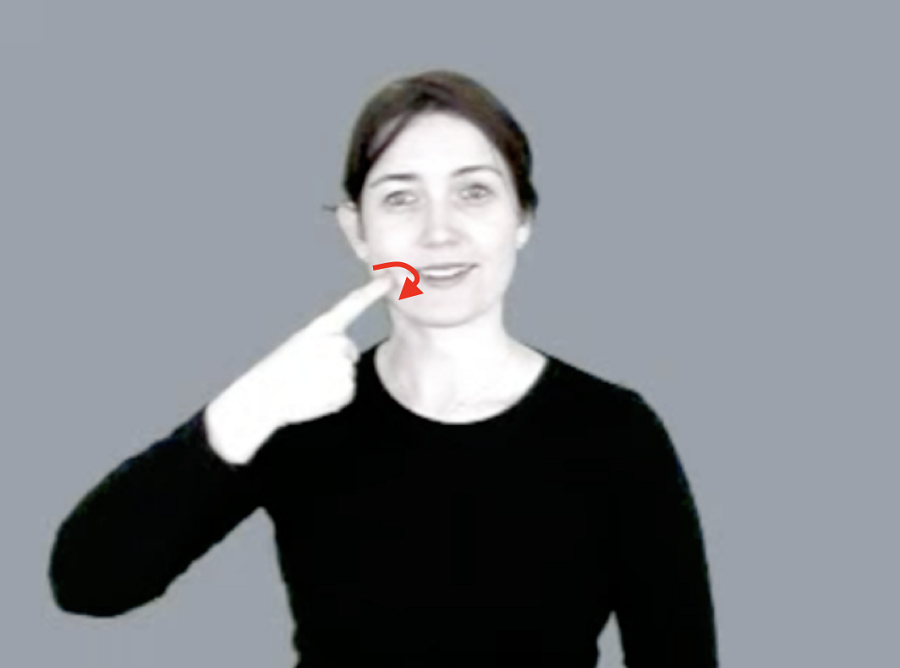
\includegraphics{../images/asl_candy.png}
\caption{CANDY}
\end{figure}

\newpage

\begin{center}
\textbf{{\color{red}{\HUGE END OF EXAM}}}\\

\end{center}
\newpage

\begin{center}
\textbf{{\color{blue}{\HUGE START OF EXAM\\}}}

\textbf{{\color{blue}{\HUGE Student ID: 3514\\}}}

\textbf{{\color{blue}{\HUGE 3:30 - 3:45 PM\\}}}

\end{center}
\newpage

{\large Question 1}\\

Source: Quiz 3, Question 1\\

L$_X$ (Language X) has three vowels, [i], [a], and [u]. It has bi-syllabic roots like Kikuyu. It does not allow non-identical high vowels to co-occur. Of the following nine logically possible vocalic sequences, which ones should be unattested in L$_X$? Explain why.\\

\begin{itemize} \item {[i...i]} \item {[i...a]} \item {[i...u]} \item {[a...i]} \item {[a...a]} \item {[a...u]} \item {[u...i]} \item {[u...a]} \item {[u...u]} \end{itemize}


\newpage

{\large Question 2}\\

Source: Day 6 Handout, Question 5\\

Is the statement given below a good description of the distribution of sounds in this dataset? Why or why not?\\

The sounds {[pʰ]} and {[p̚]} are in complementary distribution. {[pʰ]} occurs after front vowels, as in {[kæpʰ]} ‘cap,’ while {[p̚]} occurs after back vowels, as in {[tʃɑp̚]} ‘chop.’

\begin{figure}[H]
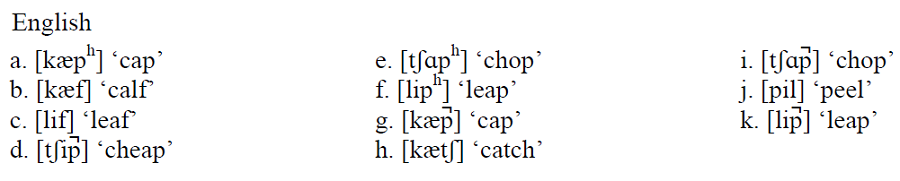
\includegraphics{../images/english_labials.png}
\end{figure}

\newpage

{\large Question 3}\\

Source: Day 6 Handout, Question 11\\

What do the two signs below tell you about the phonological status of \underline{handshape} in ASL, and why?\\

\begin{figure}[H]
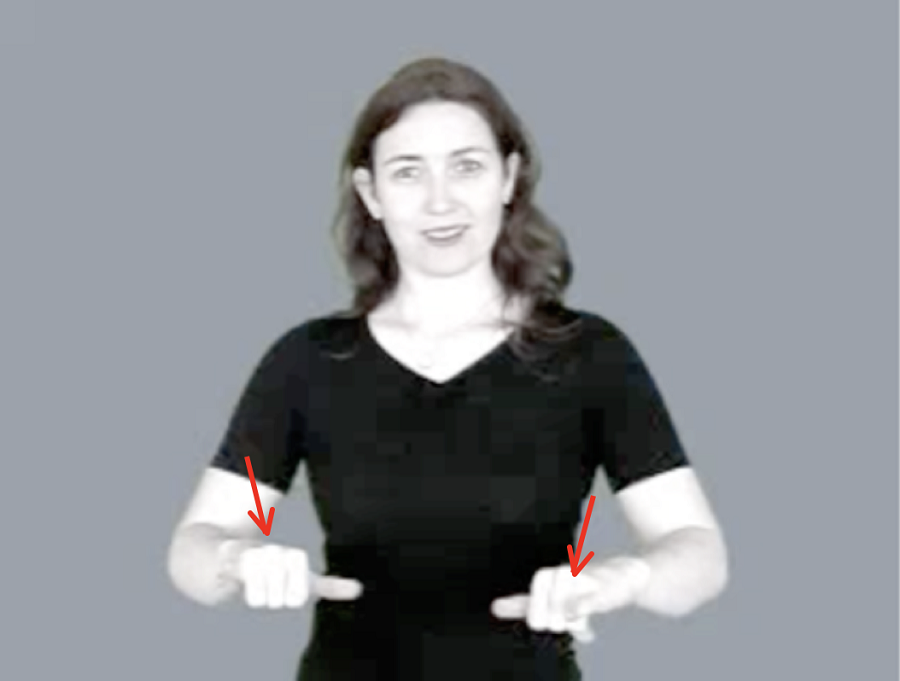
\includegraphics{../images/asl_stay.png}
\caption{STAY}
\end{figure}
\begin{figure}[H]
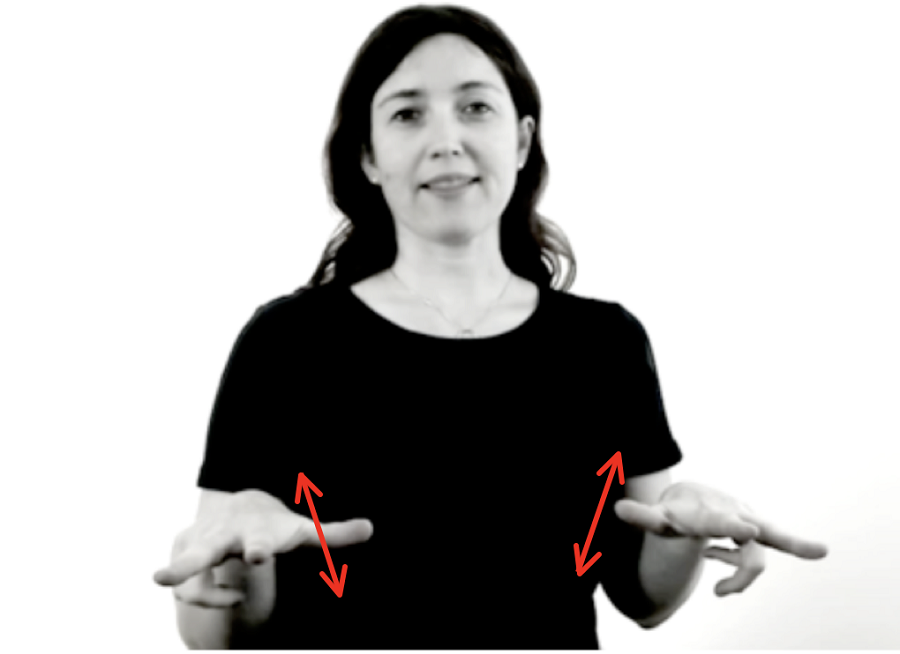
\includegraphics{../images/asl_awkward.png}
\caption{AWKWARD}
\end{figure}

\newpage

{\large Question 4}\\

Source: Day 2 Handout, Part I, Question 11\\

How would this word be transcribed?\\ Follow-up question: Why did you use symbol [X] instead of symbol [Y]?\\

<little>


\newpage

{\large Question 5}\\

Source: Day 2 Handout, Part II, Question 7\\

Is the symbol given a reasonable way to transcribe any of the sounds described below? If so, which one? If not, why not?\\

{[v]}

\begin{itemize} \item voiceless palatal affricate \item voiced velar nasal \item voiceless glottal fricative \item voiced labiodental fricative \item voiced interdental fricative \item voiced palatal fricative \end{itemize}


\newpage

\begin{center}
\textbf{{\color{red}{\HUGE END OF EXAM}}}\\

\end{center}
\newpage

\begin{center}
\textbf{{\color{blue}{\HUGE START OF EXAM\\}}}

\textbf{{\color{blue}{\HUGE Student ID: 8350\\}}}

\textbf{{\color{blue}{\HUGE 3:45 - 4:00 PM\\}}}

\end{center}
\newpage

{\large Question 1}\\

Source: Day 5 Handout, Question 3\\

What evidence is there that there is a pattern in these data, assuming that these are the only CV and VC sequences that occur in some language?\\

{[sa]}, {[ʃi]}, {[za]}, {[ʒi]}, {[as]}, {[iʃ]}, {[az]}, {[iʒ]}


\newpage

{\large Question 2}\\

Source: Day 2 Handout, Part I, Question 11\\

How would this word be transcribed?\\ Follow-up question: Why did you use symbol [X] instead of symbol [Y]?\\

<wealth>


\newpage

{\large Question 3}\\

Source: Day 2 Handout, Part II, Question 7\\

Is the symbol given a reasonable way to transcribe any of the sounds described below? If so, which one? If not, why not?\\

{[ʃ]}

\begin{itemize} \item voiceless palatal affricate \item voiced velar nasal \item voiceless glottal fricative \item voiced labiodental fricative \item voiced interdental fricative \item voiced palatal fricative \end{itemize}


\newpage

{\large Question 4}\\

Source: Day 2 Handout, Part II, Question 7\\

Is the symbol given a reasonable way to transcribe any of the sounds described below? If so, which one? If not, why not?\\

{[θ]}

\begin{itemize} \item voiceless palatal affricate \item voiced velar nasal \item voiceless glottal fricative \item voiced labiodental fricative \item voiced interdental fricative \item voiced palatal fricative \end{itemize}


\newpage

{\large Question 5}\\

Source: Day 6 Handout, Question 11\\

What do the two signs below tell you about the phonological status of \underline{handshape} in ASL, and why?\\

\begin{figure}[H]
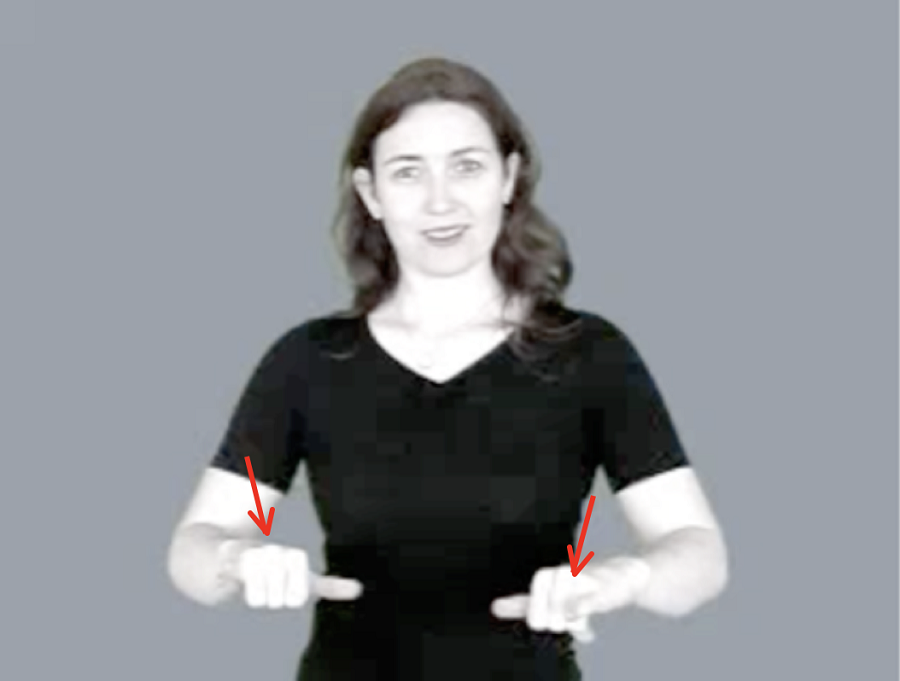
\includegraphics{../images/asl_stay.png}
\caption{STAY}
\end{figure}
\begin{figure}[H]
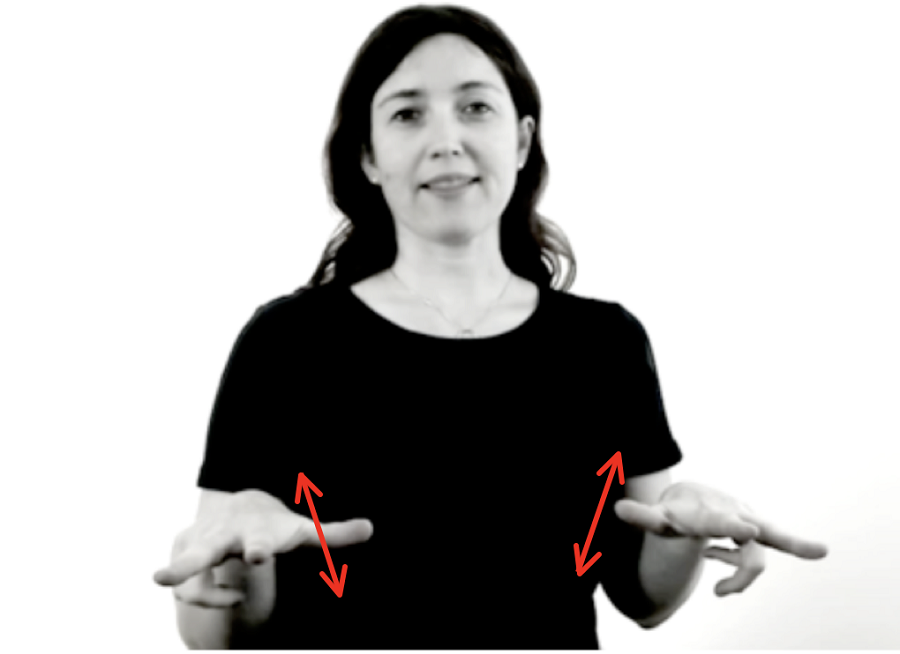
\includegraphics{../images/asl_awkward.png}
\caption{AWKWARD}
\end{figure}

\newpage

\begin{center}
\textbf{{\color{red}{\HUGE END OF EXAM}}}\\

\end{center}
\newpage

\begin{center}
\textbf{{\color{blue}{\HUGE START OF EXAM\\}}}

\textbf{{\color{blue}{\HUGE Student ID: 4090\\}}}

\textbf{{\color{blue}{\HUGE 4:00 - 4:15 PM\\}}}

\end{center}
\newpage

{\large Question 1}\\

Source: Quiz 3, Question 1\\

L$_X$ (Language X) has three vowels, [i], [a], and [u]. It has bi-syllabic roots like Kikuyu. It does not allow non-identical high vowels to co-occur. Of the following nine logically possible vocalic sequences, which ones should be unattested in L$_X$? Explain why.\\

\begin{itemize} \item {[i...i]} \item {[i...a]} \item {[i...u]} \item {[a...i]} \item {[a...a]} \item {[a...u]} \item {[u...i]} \item {[u...a]} \item {[u...u]} \end{itemize}


\newpage

{\large Question 2}\\

Source: Day 2 Handout, Part II, Question 9\\

Explain how to figure out what the sound being produced is in this diagram.\\

\begin{figure}[H]
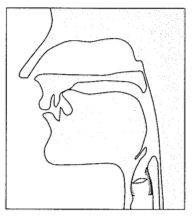
\includegraphics{../images/sagittal_t.png}
\end{figure}

\newpage

{\large Question 3}\\

Source: Homework 2, Question 1\\

What would this Klingon phrase below be in English? How do you know?\\

{[vɑdʒqʰoqʰvɑm]}

\begin{figure}[H]
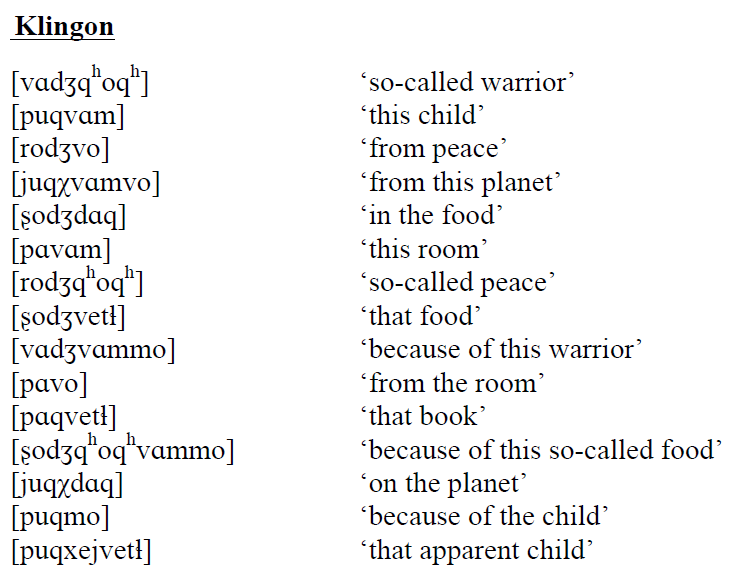
\includegraphics{../images/klingon.png}
\end{figure}

\newpage

{\large Question 4}\\

Source: Day 7 Handout, Question 9\\

What is the basic analysis of vowel length in this dataset, and what are the key pieces of evidence?\\

\begin{figure}[H]
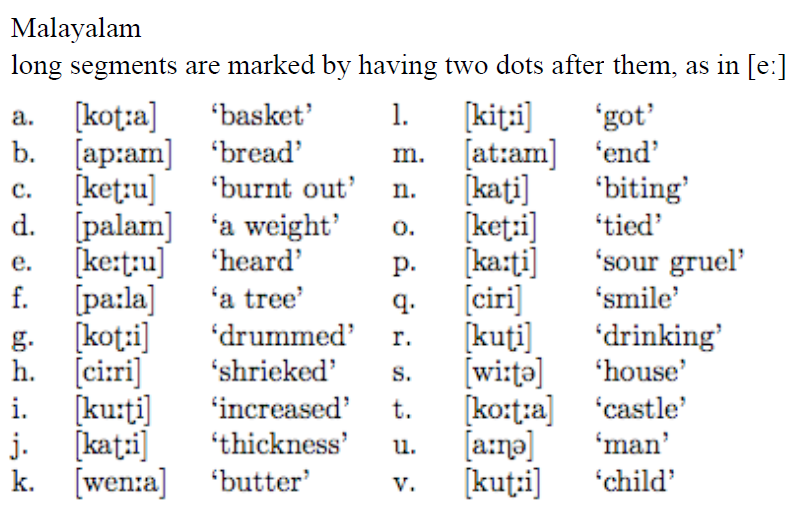
\includegraphics{../images/malayalam.png}
\end{figure}

\newpage

{\large Question 5}\\

Source: Day 2 Handout, Part I, Question 11\\

How would this word be transcribed?\\ Follow-up question: Why did you use symbol [X] instead of symbol [Y]?\\

<bird>


\newpage

\begin{center}
\textbf{{\color{red}{\HUGE END OF EXAM}}}\\

\end{center}
\newpage

\begin{center}
\textbf{{\color{blue}{\HUGE START OF EXAM\\}}}

\textbf{{\color{blue}{\HUGE Student ID: 2358\\}}}

\textbf{{\color{blue}{\HUGE 4:15 - 4:30 PM\\}}}

\end{center}
\newpage

{\large Question 1}\\

Source: Quiz 3, Question 2\\

L$_X$ has tri-syllabic roots. If L$_X$ does not allow non-identical high vowels to co-occur, which one of the following tri-syllabic vocalic sequences do you predict to be unattested in L$_X$? Explain why.\\

\begin{itemize} \item {[u...i...a]} \item {[a...i...a]} \item {[u...u...a]} \item {[a...i...i]} \end{itemize}


\newpage

{\large Question 2}\\

Source: Homework 1, Question 3(b)\\

Explain why this is or is not a complete natural class in standard North American English.\\

{[b]}, {[n]}, {[ɡ]}, {[ʒ]}, {[v]}


\newpage

{\large Question 3}\\

Source: Day 2 Handout, Part I, Question 11\\

How would this word be transcribed?\\ Follow-up question: Why did you use symbol [X] instead of symbol [Y]?\\

<toy>


\newpage

{\large Question 4}\\

Source: Day 6 Handout, Question 11\\

What do the two signs below tell you about the phonological status of \underline{handshape} in ASL, and why?\\

\begin{figure}[H]
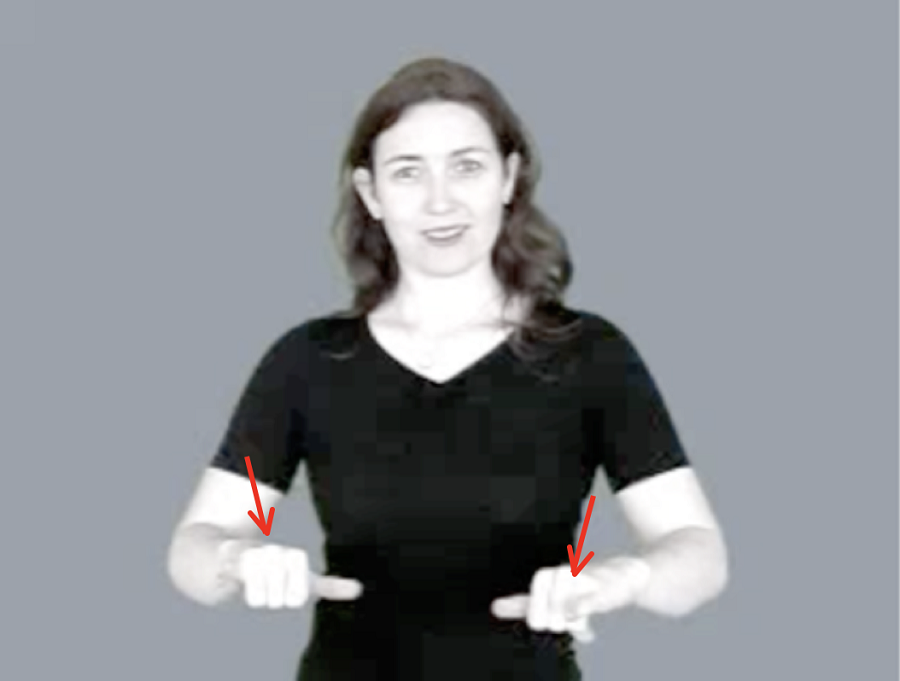
\includegraphics{../images/asl_stay.png}
\caption{STAY}
\end{figure}
\begin{figure}[H]
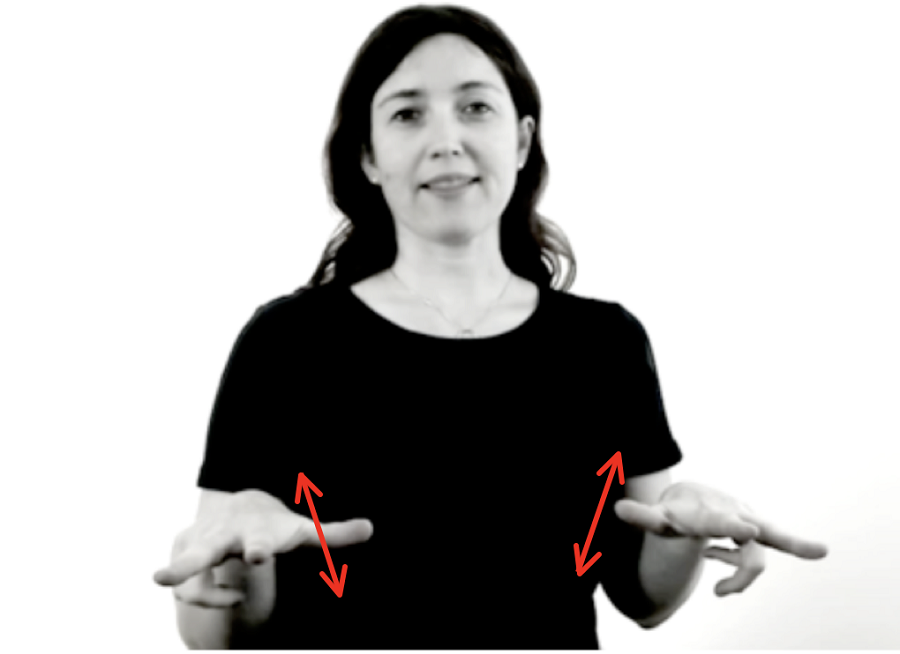
\includegraphics{../images/asl_awkward.png}
\caption{AWKWARD}
\end{figure}

\newpage

{\large Question 5}\\

Source: Homework 2, Question 1\\

What would this Klingon phrase below be in English? How do you know?\\

{[pɑdɑq]}

\begin{figure}[H]
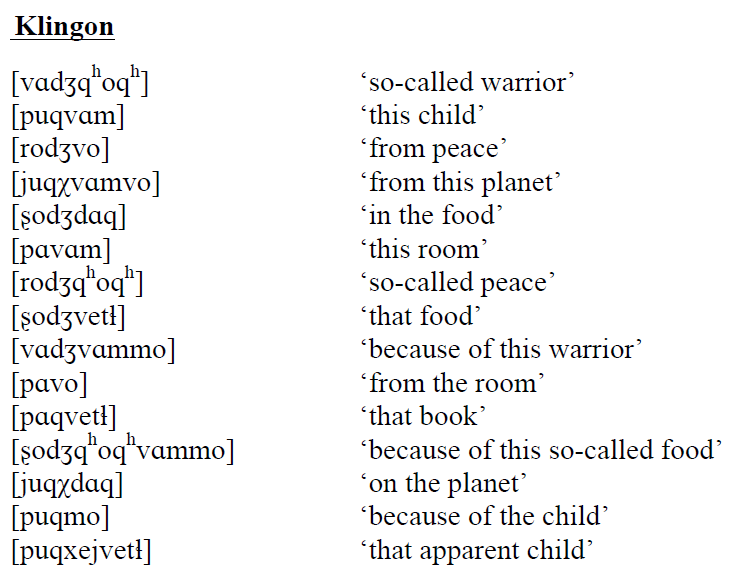
\includegraphics{../images/klingon.png}
\end{figure}

\newpage

\begin{center}
\textbf{{\color{red}{\HUGE END OF EXAM}}}\\

\end{center}
\newpage

\begin{center}
\textbf{{\color{blue}{\HUGE START OF EXAM\\}}}

\textbf{{\color{blue}{\HUGE Student ID: 9376\\}}}

\textbf{{\color{blue}{\HUGE 4:30 - 4:45 PM\\}}}

\end{center}
\newpage

{\large Question 1}\\

Source: Day 5 Handout, Question 3\\

What evidence is there that there is a pattern in these data, assuming that these are the only CV and VC sequences that occur in some language?\\

{[sa]}, {[ʃi]}, {[za]}, {[ʒi]}, {[as]}, {[iʃ]}, {[az]}, {[iʒ]}


\newpage

{\large Question 2}\\

Source: Day 2 Handout, Part I, Question 3\\

Explain why people might legitimately disagree about how many sounds this particular word contains.\\

<curtain>


\newpage

{\large Question 3}\\

Source: Day 6 Handout, Question 5\\

Explain how you would determine the phonological relationship between these two sounds (given below) in this dataset.\\

{[pʰ]} and {[f]}

\begin{figure}[H]
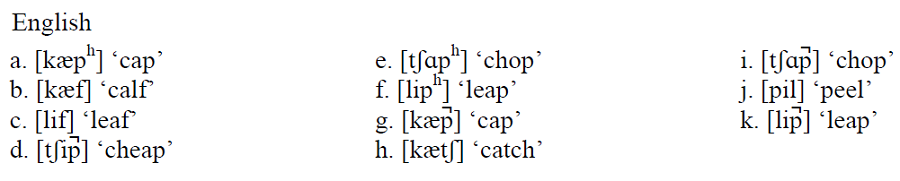
\includegraphics{../images/english_labials.png}
\end{figure}

\newpage

{\large Question 4}\\

Source: Homework 1, Question 3(a)\\

Could this image be the result of producing the sound represented by the given IPA symbol? Why or why not?\\

{[d]}

\begin{figure}[H]
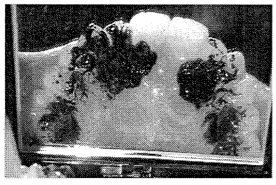
\includegraphics{../images/staticpalatography_fricative.png}
\end{figure}

\newpage

{\large Question 5}\\

Source: Day 6 Handout, Question 11\\

What do the two signs below tell you about the phonological status of \underline{handshape} in ASL, and why?\\

\begin{figure}[H]
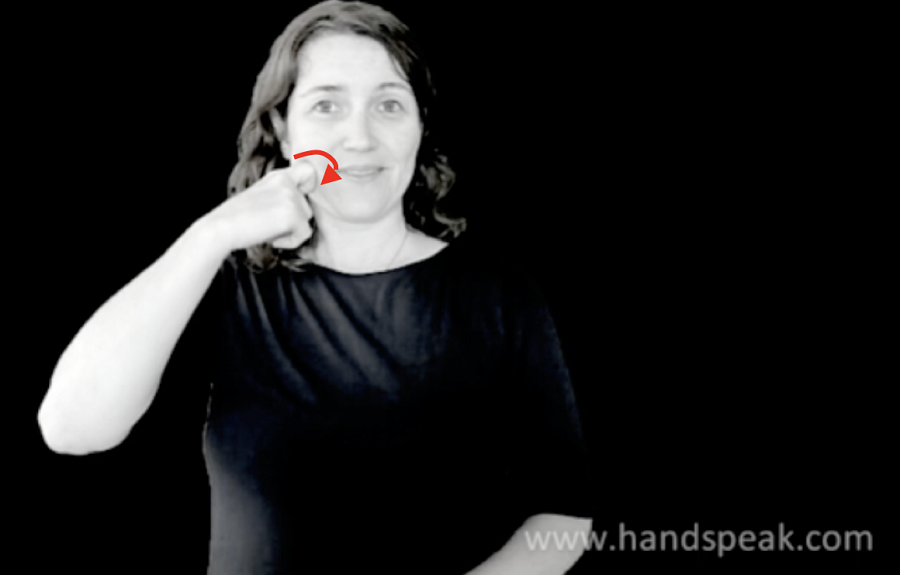
\includegraphics{../images/asl_apple.png}
\caption{APPLE}
\end{figure}
\begin{figure}[H]
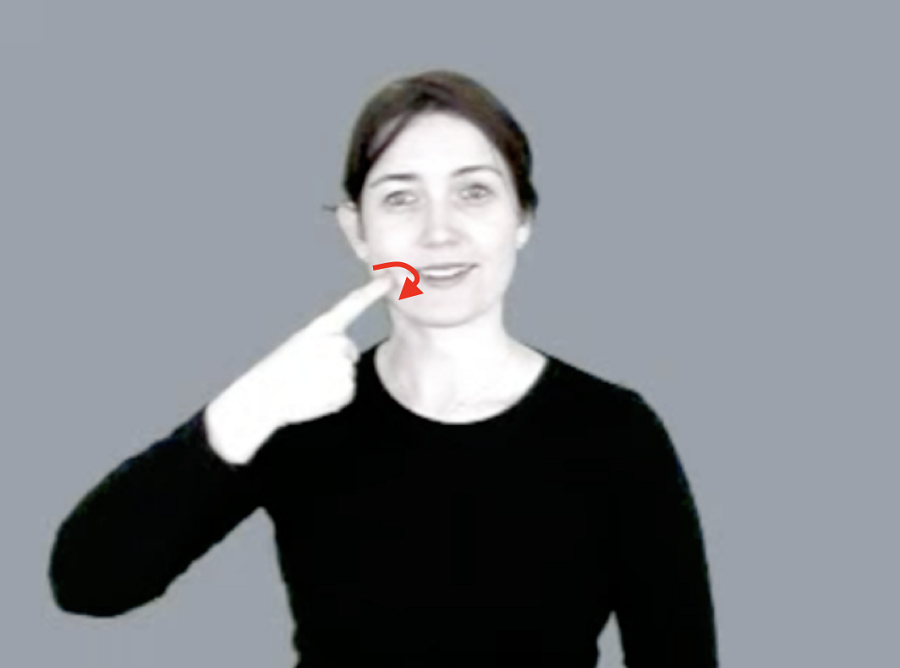
\includegraphics{../images/asl_candy.png}
\caption{CANDY}
\end{figure}

\newpage

\begin{center}
\textbf{{\color{red}{\HUGE END OF EXAM}}}\\

\end{center}
\newpage

\end{document}

